% Options for packages loaded elsewhere
% Options for packages loaded elsewhere
\PassOptionsToPackage{unicode}{hyperref}
\PassOptionsToPackage{hyphens}{url}
\PassOptionsToPackage{dvipsnames,svgnames,x11names}{xcolor}
%
\documentclass[
  ngerman,
]{article}
\usepackage{xcolor}
\usepackage[margin=2cm]{geometry}
\usepackage{amsmath,amssymb}
\setcounter{secnumdepth}{-\maxdimen} % remove section numbering
\usepackage{iftex}
\ifPDFTeX
  \usepackage[T1]{fontenc}
  \usepackage[utf8]{inputenc}
  \usepackage{textcomp} % provide euro and other symbols
\else % if luatex or xetex
  \usepackage{unicode-math} % this also loads fontspec
  \defaultfontfeatures{Scale=MatchLowercase}
  \defaultfontfeatures[\rmfamily]{Ligatures=TeX,Scale=1}
\fi
\usepackage{lmodern}
\ifPDFTeX\else
  % xetex/luatex font selection
\fi
% Use upquote if available, for straight quotes in verbatim environments
\IfFileExists{upquote.sty}{\usepackage{upquote}}{}
\IfFileExists{microtype.sty}{% use microtype if available
  \usepackage[]{microtype}
  \UseMicrotypeSet[protrusion]{basicmath} % disable protrusion for tt fonts
}{}
\makeatletter
\@ifundefined{KOMAClassName}{% if non-KOMA class
  \IfFileExists{parskip.sty}{%
    \usepackage{parskip}
  }{% else
    \setlength{\parindent}{0pt}
    \setlength{\parskip}{6pt plus 2pt minus 1pt}}
}{% if KOMA class
  \KOMAoptions{parskip=half}}
\makeatother
% Make \paragraph and \subparagraph free-standing
\makeatletter
\ifx\paragraph\undefined\else
  \let\oldparagraph\paragraph
  \renewcommand{\paragraph}{
    \@ifstar
      \xxxParagraphStar
      \xxxParagraphNoStar
  }
  \newcommand{\xxxParagraphStar}[1]{\oldparagraph*{#1}\mbox{}}
  \newcommand{\xxxParagraphNoStar}[1]{\oldparagraph{#1}\mbox{}}
\fi
\ifx\subparagraph\undefined\else
  \let\oldsubparagraph\subparagraph
  \renewcommand{\subparagraph}{
    \@ifstar
      \xxxSubParagraphStar
      \xxxSubParagraphNoStar
  }
  \newcommand{\xxxSubParagraphStar}[1]{\oldsubparagraph*{#1}\mbox{}}
  \newcommand{\xxxSubParagraphNoStar}[1]{\oldsubparagraph{#1}\mbox{}}
\fi
\makeatother

\usepackage{color}
\usepackage{fancyvrb}
\newcommand{\VerbBar}{|}
\newcommand{\VERB}{\Verb[commandchars=\\\{\}]}
\DefineVerbatimEnvironment{Highlighting}{Verbatim}{commandchars=\\\{\}}
% Add ',fontsize=\small' for more characters per line
\usepackage{framed}
\definecolor{shadecolor}{RGB}{241,243,245}
\newenvironment{Shaded}{\begin{snugshade}}{\end{snugshade}}
\newcommand{\AlertTok}[1]{\textcolor[rgb]{0.68,0.00,0.00}{#1}}
\newcommand{\AnnotationTok}[1]{\textcolor[rgb]{0.37,0.37,0.37}{#1}}
\newcommand{\AttributeTok}[1]{\textcolor[rgb]{0.40,0.45,0.13}{#1}}
\newcommand{\BaseNTok}[1]{\textcolor[rgb]{0.68,0.00,0.00}{#1}}
\newcommand{\BuiltInTok}[1]{\textcolor[rgb]{0.00,0.23,0.31}{#1}}
\newcommand{\CharTok}[1]{\textcolor[rgb]{0.13,0.47,0.30}{#1}}
\newcommand{\CommentTok}[1]{\textcolor[rgb]{0.37,0.37,0.37}{#1}}
\newcommand{\CommentVarTok}[1]{\textcolor[rgb]{0.37,0.37,0.37}{\textit{#1}}}
\newcommand{\ConstantTok}[1]{\textcolor[rgb]{0.56,0.35,0.01}{#1}}
\newcommand{\ControlFlowTok}[1]{\textcolor[rgb]{0.00,0.23,0.31}{\textbf{#1}}}
\newcommand{\DataTypeTok}[1]{\textcolor[rgb]{0.68,0.00,0.00}{#1}}
\newcommand{\DecValTok}[1]{\textcolor[rgb]{0.68,0.00,0.00}{#1}}
\newcommand{\DocumentationTok}[1]{\textcolor[rgb]{0.37,0.37,0.37}{\textit{#1}}}
\newcommand{\ErrorTok}[1]{\textcolor[rgb]{0.68,0.00,0.00}{#1}}
\newcommand{\ExtensionTok}[1]{\textcolor[rgb]{0.00,0.23,0.31}{#1}}
\newcommand{\FloatTok}[1]{\textcolor[rgb]{0.68,0.00,0.00}{#1}}
\newcommand{\FunctionTok}[1]{\textcolor[rgb]{0.28,0.35,0.67}{#1}}
\newcommand{\ImportTok}[1]{\textcolor[rgb]{0.00,0.46,0.62}{#1}}
\newcommand{\InformationTok}[1]{\textcolor[rgb]{0.37,0.37,0.37}{#1}}
\newcommand{\KeywordTok}[1]{\textcolor[rgb]{0.00,0.23,0.31}{\textbf{#1}}}
\newcommand{\NormalTok}[1]{\textcolor[rgb]{0.00,0.23,0.31}{#1}}
\newcommand{\OperatorTok}[1]{\textcolor[rgb]{0.37,0.37,0.37}{#1}}
\newcommand{\OtherTok}[1]{\textcolor[rgb]{0.00,0.23,0.31}{#1}}
\newcommand{\PreprocessorTok}[1]{\textcolor[rgb]{0.68,0.00,0.00}{#1}}
\newcommand{\RegionMarkerTok}[1]{\textcolor[rgb]{0.00,0.23,0.31}{#1}}
\newcommand{\SpecialCharTok}[1]{\textcolor[rgb]{0.37,0.37,0.37}{#1}}
\newcommand{\SpecialStringTok}[1]{\textcolor[rgb]{0.13,0.47,0.30}{#1}}
\newcommand{\StringTok}[1]{\textcolor[rgb]{0.13,0.47,0.30}{#1}}
\newcommand{\VariableTok}[1]{\textcolor[rgb]{0.07,0.07,0.07}{#1}}
\newcommand{\VerbatimStringTok}[1]{\textcolor[rgb]{0.13,0.47,0.30}{#1}}
\newcommand{\WarningTok}[1]{\textcolor[rgb]{0.37,0.37,0.37}{\textit{#1}}}

\usepackage{longtable,booktabs,array}
\newcounter{none} % for unnumbered tables
\usepackage{calc} % for calculating minipage widths
% Correct order of tables after \paragraph or \subparagraph
\usepackage{etoolbox}
\makeatletter
\patchcmd\longtable{\par}{\if@noskipsec\mbox{}\fi\par}{}{}
\makeatother
% Allow footnotes in longtable head/foot
\IfFileExists{footnotehyper.sty}{\usepackage{footnotehyper}}{\usepackage{footnote}}
\makesavenoteenv{longtable}
\usepackage{graphicx}
\makeatletter
\newsavebox\pandoc@box
\newcommand*\pandocbounded[1]{% scales image to fit in text height/width
  \sbox\pandoc@box{#1}%
  \Gscale@div\@tempa{\textheight}{\dimexpr\ht\pandoc@box+\dp\pandoc@box\relax}%
  \Gscale@div\@tempb{\linewidth}{\wd\pandoc@box}%
  \ifdim\@tempb\p@<\@tempa\p@\let\@tempa\@tempb\fi% select the smaller of both
  \ifdim\@tempa\p@<\p@\scalebox{\@tempa}{\usebox\pandoc@box}%
  \else\usebox{\pandoc@box}%
  \fi%
}
% Set default figure placement to htbp
\def\fps@figure{htbp}
\makeatother



\ifLuaTeX
\usepackage[bidi=basic,shorthands=off]{babel}
\else
\usepackage[bidi=default,shorthands=off]{babel}
\fi
\ifLuaTeX
  \usepackage{selnolig} % disable illegal ligatures
\fi


\setlength{\emergencystretch}{3em} % prevent overfull lines

\providecommand{\tightlist}{%
  \setlength{\itemsep}{0pt}\setlength{\parskip}{0pt}}



 


\makeatletter
\@ifpackageloaded{caption}{}{\usepackage{caption}}
\AtBeginDocument{%
\ifdefined\contentsname
  \renewcommand*\contentsname{Inhaltsverzeichnis}
\else
  \newcommand\contentsname{Inhaltsverzeichnis}
\fi
\ifdefined\listfigurename
  \renewcommand*\listfigurename{Abbildungsverzeichnis}
\else
  \newcommand\listfigurename{Abbildungsverzeichnis}
\fi
\ifdefined\listtablename
  \renewcommand*\listtablename{Tabellenverzeichnis}
\else
  \newcommand\listtablename{Tabellenverzeichnis}
\fi
\ifdefined\figurename
  \renewcommand*\figurename{Abbildung}
\else
  \newcommand\figurename{Abbildung}
\fi
\ifdefined\tablename
  \renewcommand*\tablename{Tabelle}
\else
  \newcommand\tablename{Tabelle}
\fi
}
\@ifpackageloaded{float}{}{\usepackage{float}}
\floatstyle{ruled}
\@ifundefined{c@chapter}{\newfloat{codelisting}{h}{lop}}{\newfloat{codelisting}{h}{lop}[chapter]}
\floatname{codelisting}{Listing}
\newcommand*\listoflistings{\listof{codelisting}{Listingverzeichnis}}
\makeatother
\makeatletter
\makeatother
\makeatletter
\@ifpackageloaded{caption}{}{\usepackage{caption}}
\@ifpackageloaded{subcaption}{}{\usepackage{subcaption}}
\makeatother
\usepackage{bookmark}
\IfFileExists{xurl.sty}{\usepackage{xurl}}{} % add URL line breaks if available
\urlstyle{same}
\hypersetup{
  pdftitle={CSG --- Mathematischer Deep Dive},
  pdfauthor={Moritz Potthoff},
  pdflang={de},
  colorlinks=true,
  linkcolor={blue},
  filecolor={Maroon},
  citecolor={Blue},
  urlcolor={Blue},
  pdfcreator={LaTeX via pandoc}}


\title{CSG --- Mathematischer Deep Dive}
\usepackage{etoolbox}
\makeatletter
\providecommand{\subtitle}[1]{% add subtitle to \maketitle
  \apptocmd{\@title}{\par {\large #1 \par}}{}{}
}
\makeatother
\subtitle{Folgeseiten (Entwurf) · Moritz Potthoff}
\author{Moritz Potthoff}
\date{2026-06-17}
\begin{document}
\maketitle


\section{Kontext}\label{kontext}

\subsection{Was wir bereits wissen}\label{was-wir-bereits-wissen}

\begin{itemize}
\tightlist
\item
  \textbf{SDF:} \(f:\mathbb{R}^3\to\mathbb{R}\) --- negativ innen, null
  auf der Fläche, positiv außen
\item
  \textbf{Ray Marching:} entlang des Strahls mit Schrittweite
  \(|f(\mathbf{p})|\) zur Oberfläche
\item
  \textbf{Primitive:} Kugel, Box, Zylinder, \ldots{} als geschlossene
  Formeln
\end{itemize}

\vspace{0.6em}

\textbf{Diese Folien:} Wie wird aus Primitiven eine Szene --- rein
algebraisch?

\section{Von Mengen zu Distanzen}\label{von-mengen-zu-distanzen}

\subsection{Boolesche Geometrie}\label{boolesche-geometrie}

Komplexe Körper als Kombination von Grundkörpern \(A, B, C, \ldots\):

{\def\LTcaptype{none} % do not increment counter
\begin{longtable}[]{@{}lll@{}}
\toprule\noalign{}
Operation & Mengenschreibweise & Intuition \\
\midrule\noalign{}
\endhead
\bottomrule\noalign{}
\endlastfoot
Vereinigung & \(A \cup B\) & alles, was in \(A\) \textbf{oder} \(B\)
liegt \\
Schnittmenge & \(A \cap B\) & nur der \textbf{gemeinsame} Bereich \\
Differenz & \(A \setminus B\) & \(A\) \textbf{ohne} \(B\) \\
\end{longtable}
}

\vspace{0.4em}

Bei \textbf{Meshes} werden Dreiecke geschnitten --- teuer und
fehleranfällig.

Bei \textbf{SDFs} reicht eine Kombination der Distanzwerte pro Punkt
\(\mathbf{p}\).

\subsection{Venn-Diagramme →
SDF-Formeln}\label{venn-diagramme-sdf-formeln}

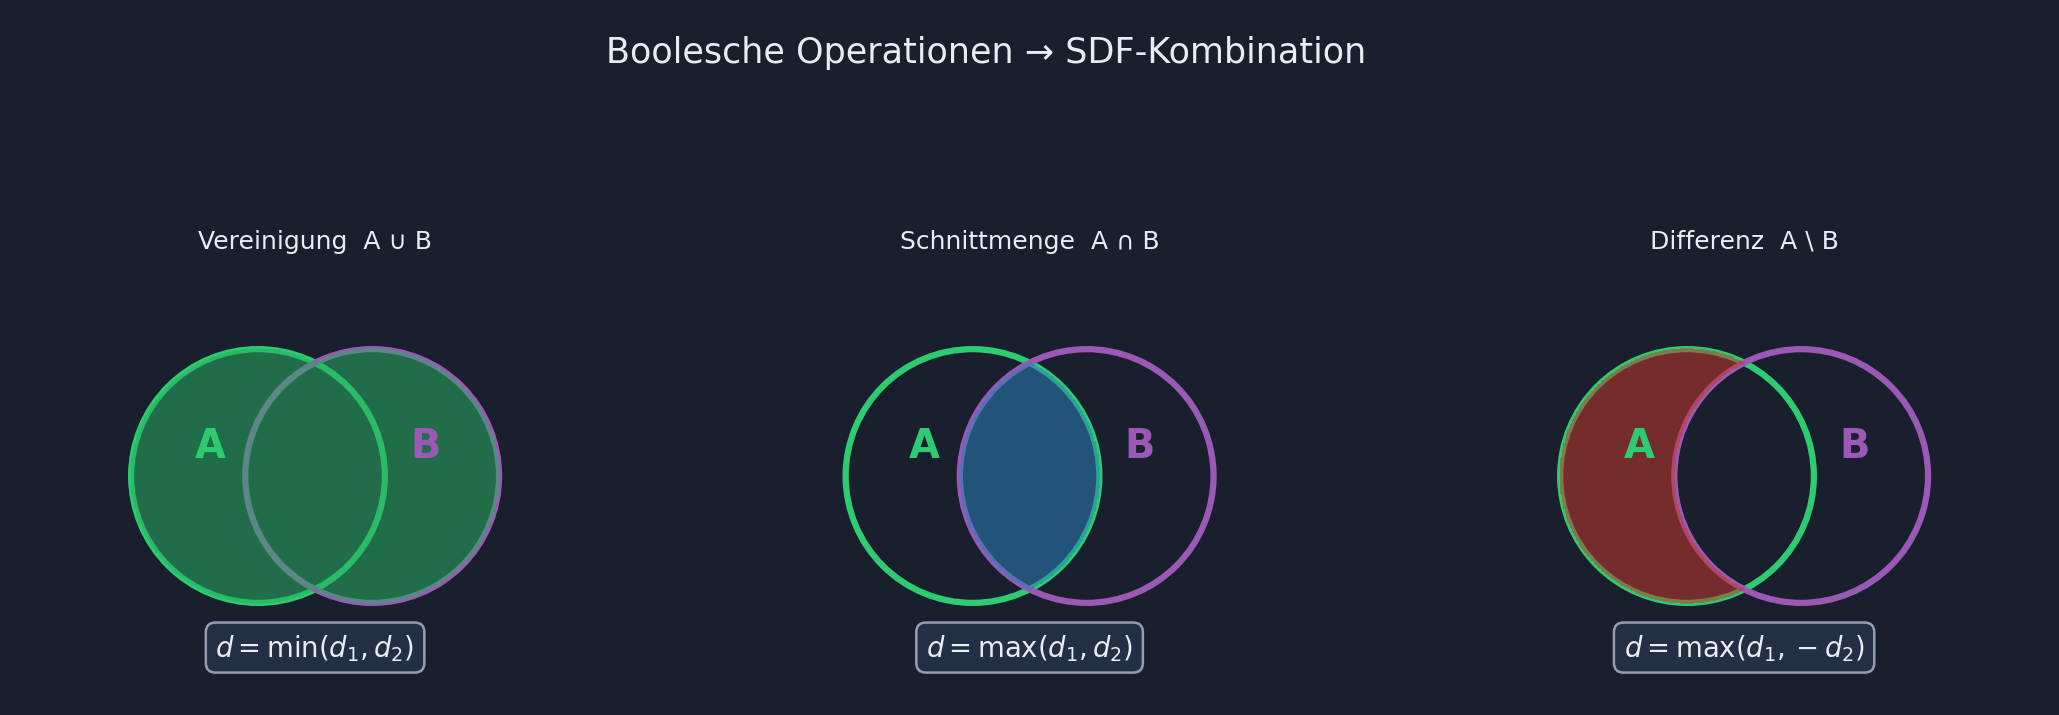
\includegraphics[width=1\linewidth,height=\textheight,keepaspectratio]{assets/diagrams/01-boolean-venn.png}

\section{Die drei Kernoperationen}\label{die-drei-kernoperationen}

\subsection{Algebraische Definition}\label{algebraische-definition}

Für zwei SDFs \(d_1(\mathbf{p})\), \(d_2(\mathbf{p})\):

\begin{align*}
\text{Union:}        \quad d(\mathbf{p}) &= \min\bigl(d_1(\mathbf{p}), d_2(\mathbf{p})\bigr) \\
\text{Intersection:}\quad d(\mathbf{p}) &= \max\bigl(d_1(\mathbf{p}), d_2(\mathbf{p})\bigr) \\
\text{Difference:}   \quad d(\mathbf{p}) &= \max\bigl(d_1(\mathbf{p}), -d_2(\mathbf{p})\bigr)
\end{align*}

\vspace{0.3em}

\textbf{Differenz-Trick:} \(-d_2\) spiegelt innen/außen von \(B\) ---
das „Herausschneiden'' wird zu einem Maximum.

\subsection{GLSL-Implementierung}\label{glsl-implementierung}

\begin{Shaded}
\begin{Highlighting}[]
\DataTypeTok{float} \FunctionTok{opUnion}\OperatorTok{(}\DataTypeTok{float}\NormalTok{ d1}\OperatorTok{,} \DataTypeTok{float}\NormalTok{ d2}\OperatorTok{)}    \OperatorTok{\{} \KeywordTok{return} \BuiltInTok{min}\OperatorTok{(}\NormalTok{d1}\OperatorTok{,}\NormalTok{ d2}\OperatorTok{);} \OperatorTok{\}}
\DataTypeTok{float} \FunctionTok{opIntersect}\OperatorTok{(}\DataTypeTok{float}\NormalTok{ d1}\OperatorTok{,} \DataTypeTok{float}\NormalTok{ d2}\OperatorTok{)\{} \KeywordTok{return} \BuiltInTok{max}\OperatorTok{(}\NormalTok{d1}\OperatorTok{,}\NormalTok{ d2}\OperatorTok{);} \OperatorTok{\}}
\DataTypeTok{float} \FunctionTok{opSubtract}\OperatorTok{(}\DataTypeTok{float}\NormalTok{ d1}\OperatorTok{,} \DataTypeTok{float}\NormalTok{ d2}\OperatorTok{)} \OperatorTok{\{} \KeywordTok{return} \BuiltInTok{max}\OperatorTok{(}\NormalTok{d1}\OperatorTok{,} \OperatorTok{{-}}\NormalTok{d2}\OperatorTok{);} \OperatorTok{\}}
\end{Highlighting}
\end{Shaded}

\vspace{0.4em}

Die gesamte Szene ist eine \textbf{verschachtelte
Ausdrucksbaum-Auswertung} --- kein neues Mesh, keine Topologie-Änderung
zur Laufzeit.

\section{Warum funktioniert das?}\label{warum-funktioniert-das}

\subsection{Innen/Außen-Logik}\label{innenauuxdfen-logik}

Ein Punkt liegt \textbf{innen}, wenn \(d < 0\) (genug negativ = tief im
Körper).

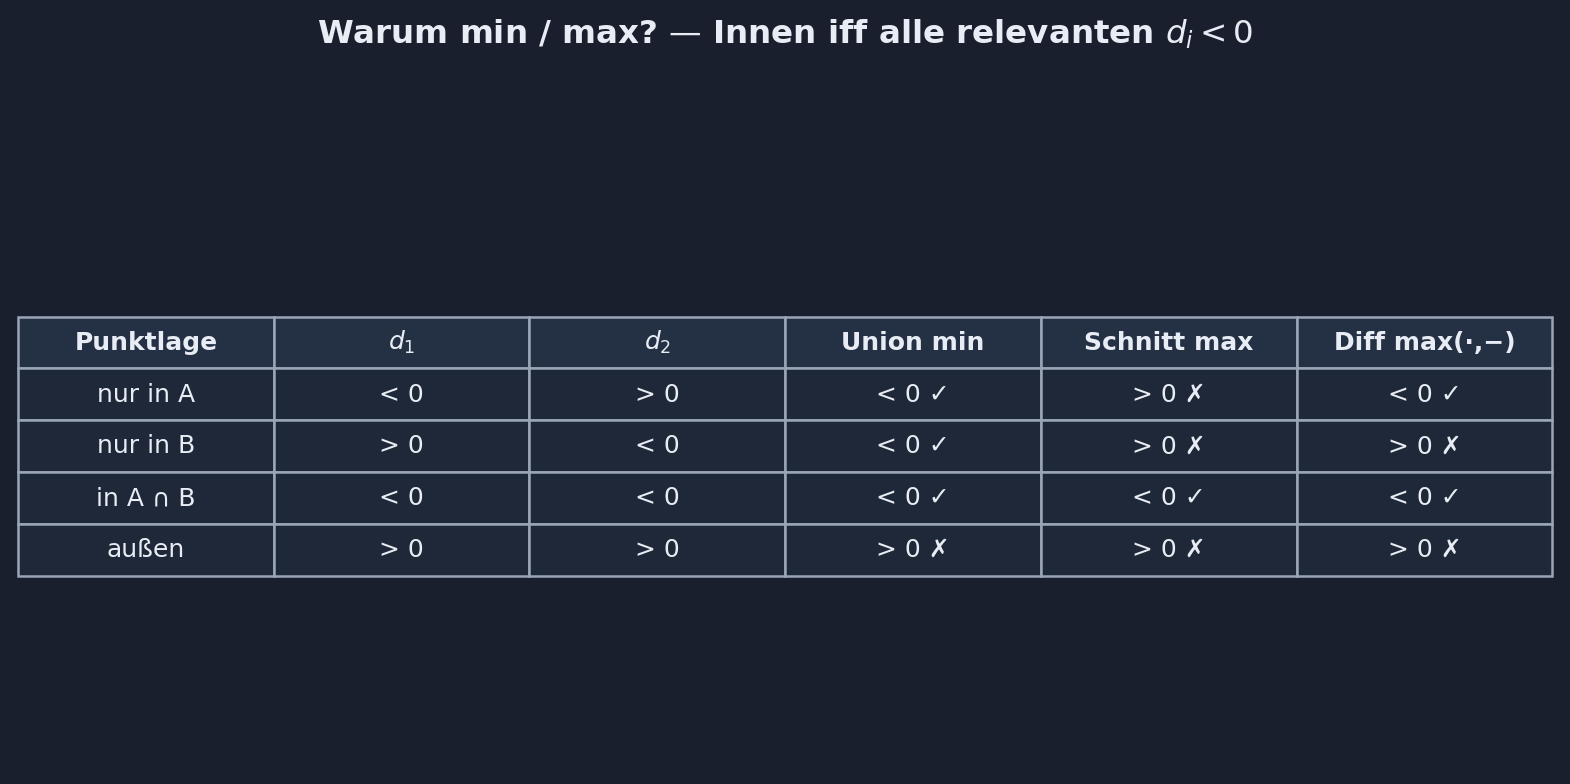
\includegraphics[width=0.92\linewidth,height=\textheight,keepaspectratio]{assets/diagrams/04-inside-outside-table.png}

\vspace{0.2em}

\small

\begin{itemize}
\tightlist
\item
  \textbf{Union:} min wählt die \emph{nähere} Fläche → innen, wenn
  \emph{mindestens eine} Form innen ist
\item
  \textbf{Schnitt:} max verlangt, dass \emph{beide} Distanzen negativ
  sind
\item
  \textbf{Differenz:} \(-d_2\) kehrt \(B\) um --- innen in \(A\), aber
  außerhalb von \(B\)
\end{itemize}

\subsection{1D-Scanline: min / max sichtbar
machen}\label{d-scanline-min-max-sichtbar-machen}

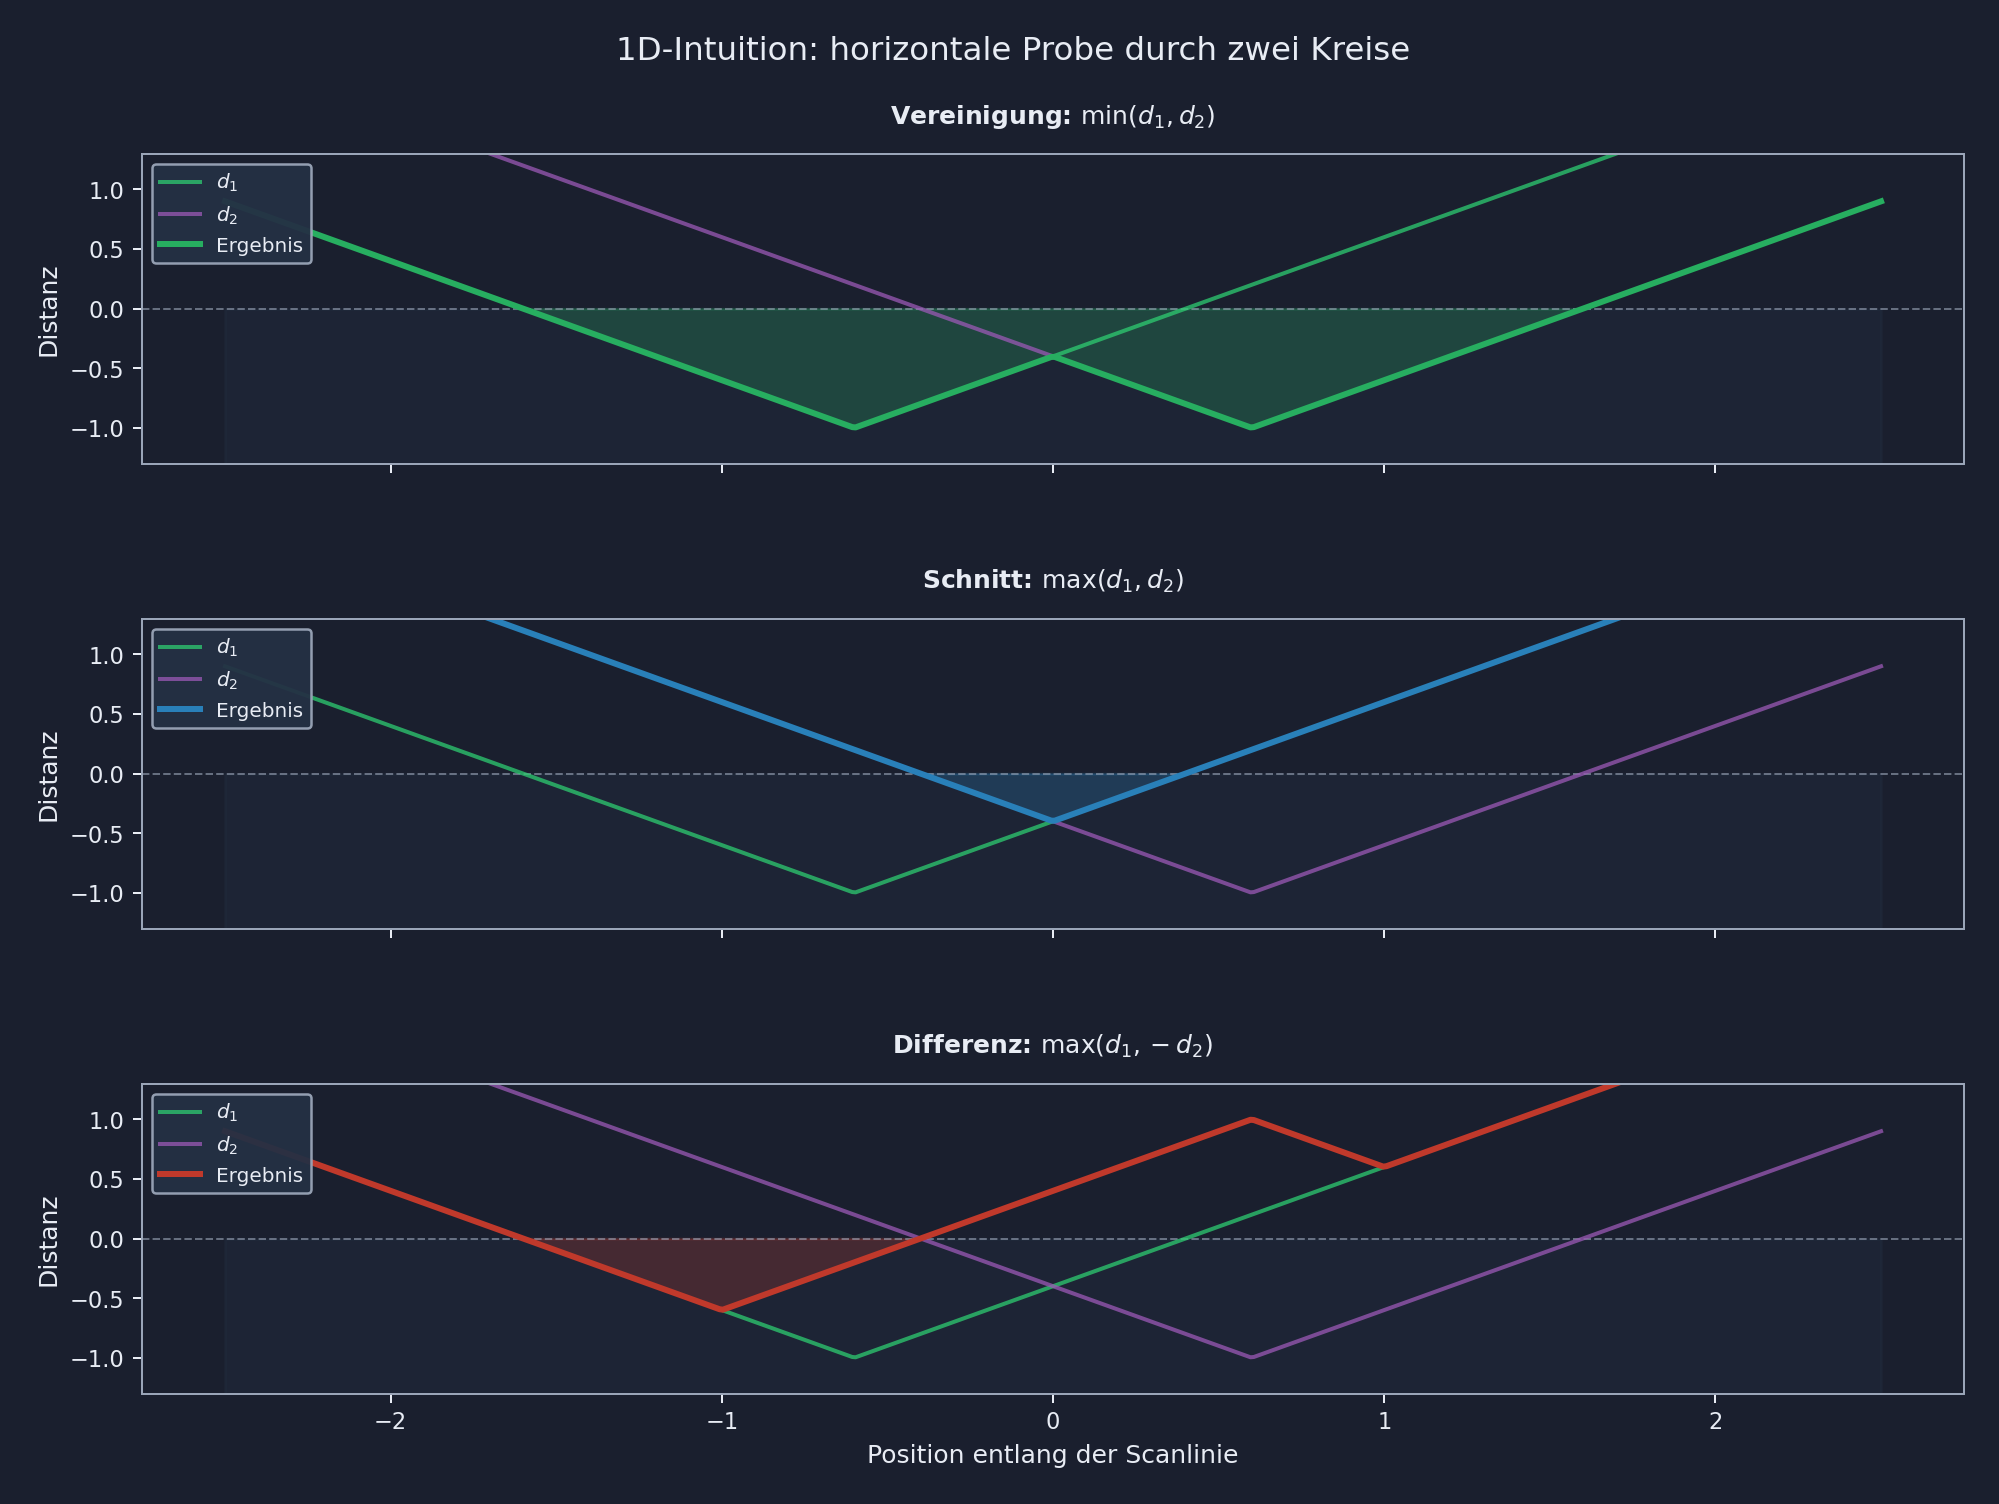
\includegraphics[width=1\linewidth,height=\textheight,keepaspectratio]{assets/diagrams/03-1d-scanline.png}

\footnotesize

Horizontale Probe durch zwei Kreise: \(d_1\), \(d_2\) und das
kombinierte Feld. Rot schattiert = \(d \le 0\) (innen).

\section{Visuell im 2D-Feld}\label{visuell-im-2d-feld}

\subsection{Distanzfelder vor und nach
CSG}\label{distanzfelder-vor-und-nach-csg}

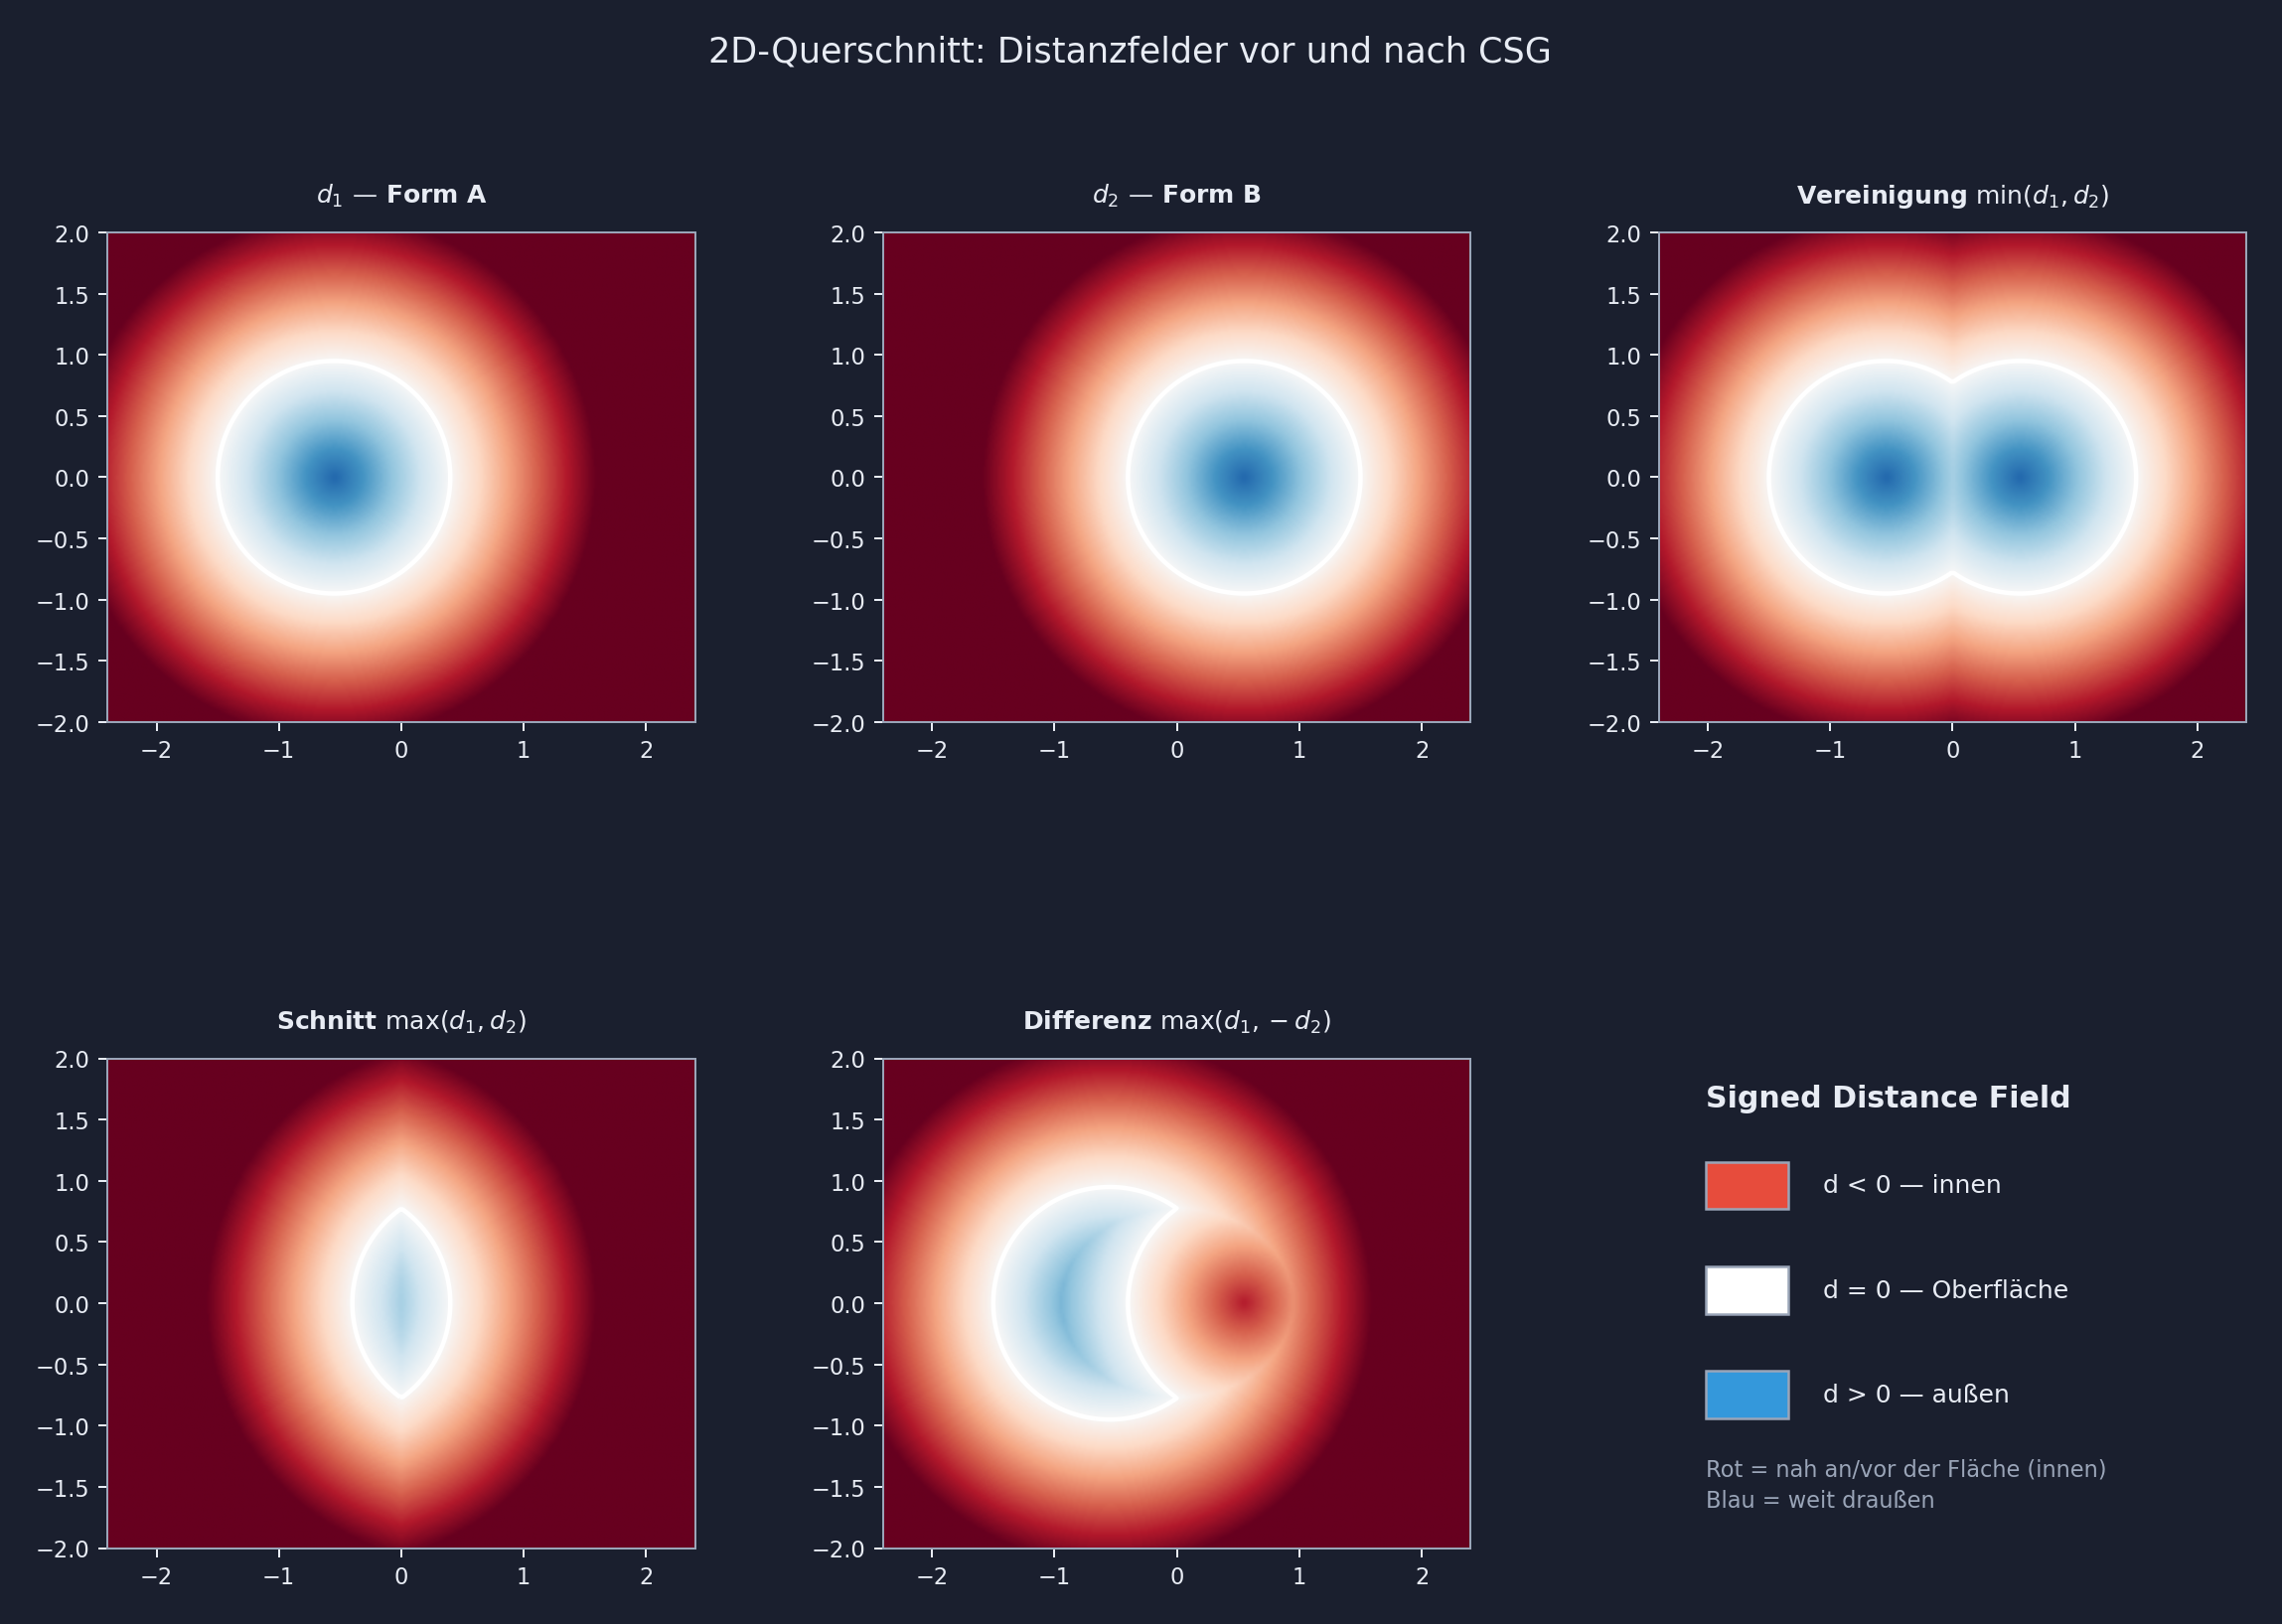
\includegraphics[width=1\linewidth,height=\textheight,keepaspectratio]{assets/diagrams/02-sdf-heatmap-panel.png}

\footnotesize

Weiße Kontur = Nullniveau (\(d=0\)) = Oberfläche. Gleiche Operationen
funktionieren in 3D --- nur die Formeln der Primitive ändern sich.

\section{CSG als Baum}\label{csg-als-baum}

\subsection{Hierarchische
Konstruktion}\label{hierarchische-konstruktion}

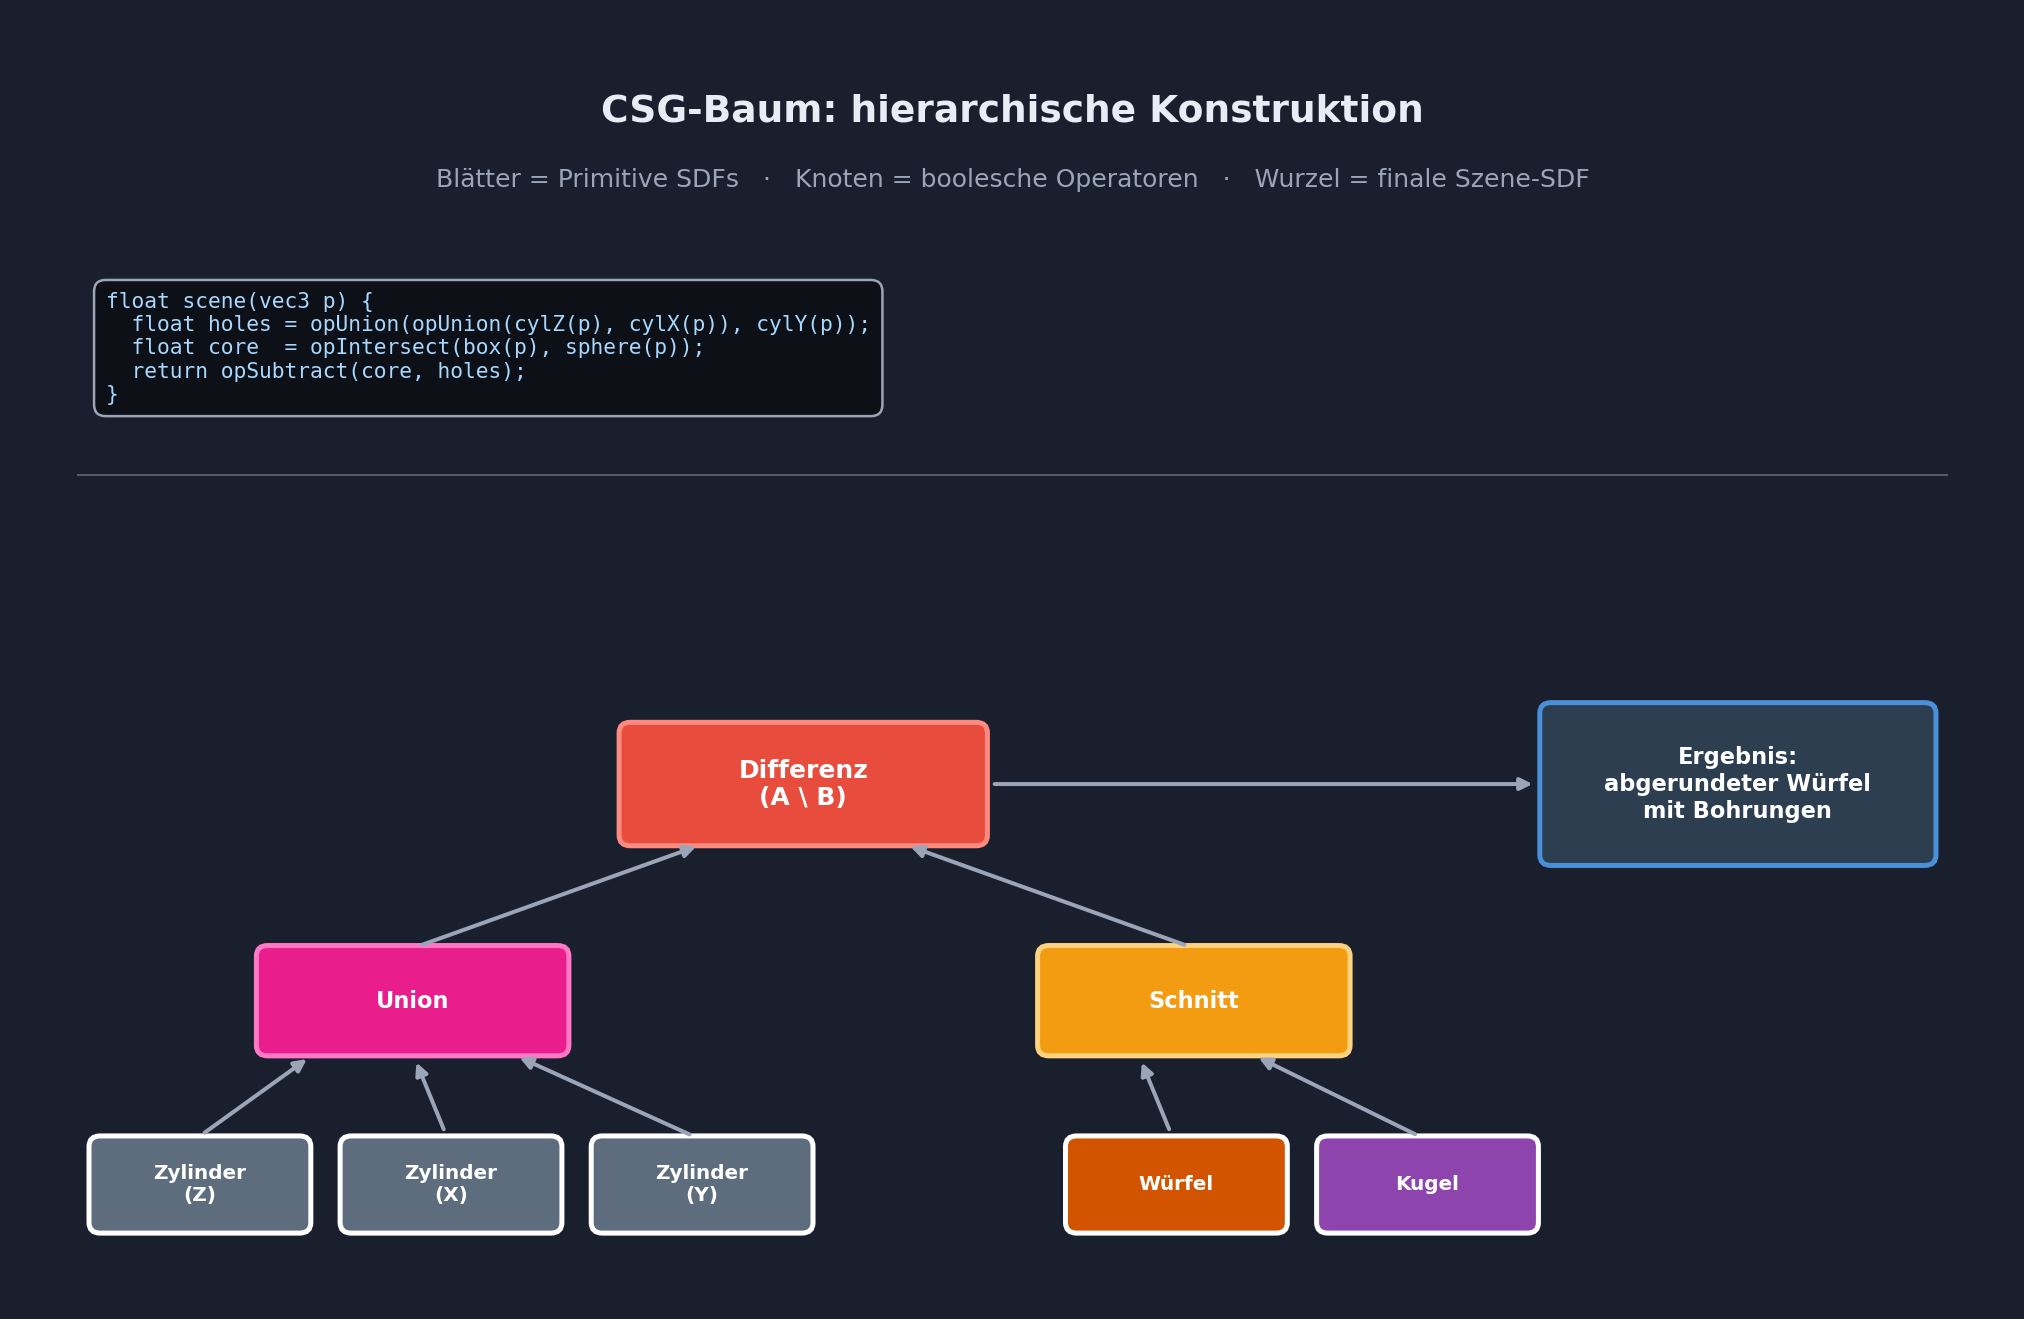
\includegraphics[width=1\linewidth,height=\textheight,keepaspectratio]{assets/diagrams/05-csg-tree.png}

\footnotesize

Blätter = Primitive · innere Knoten = Operatoren · Wurzel =
\texttt{scene(p)} für Ray Marching

\subsection{N-äre Operationen}\label{n-uxe4re-operationen}

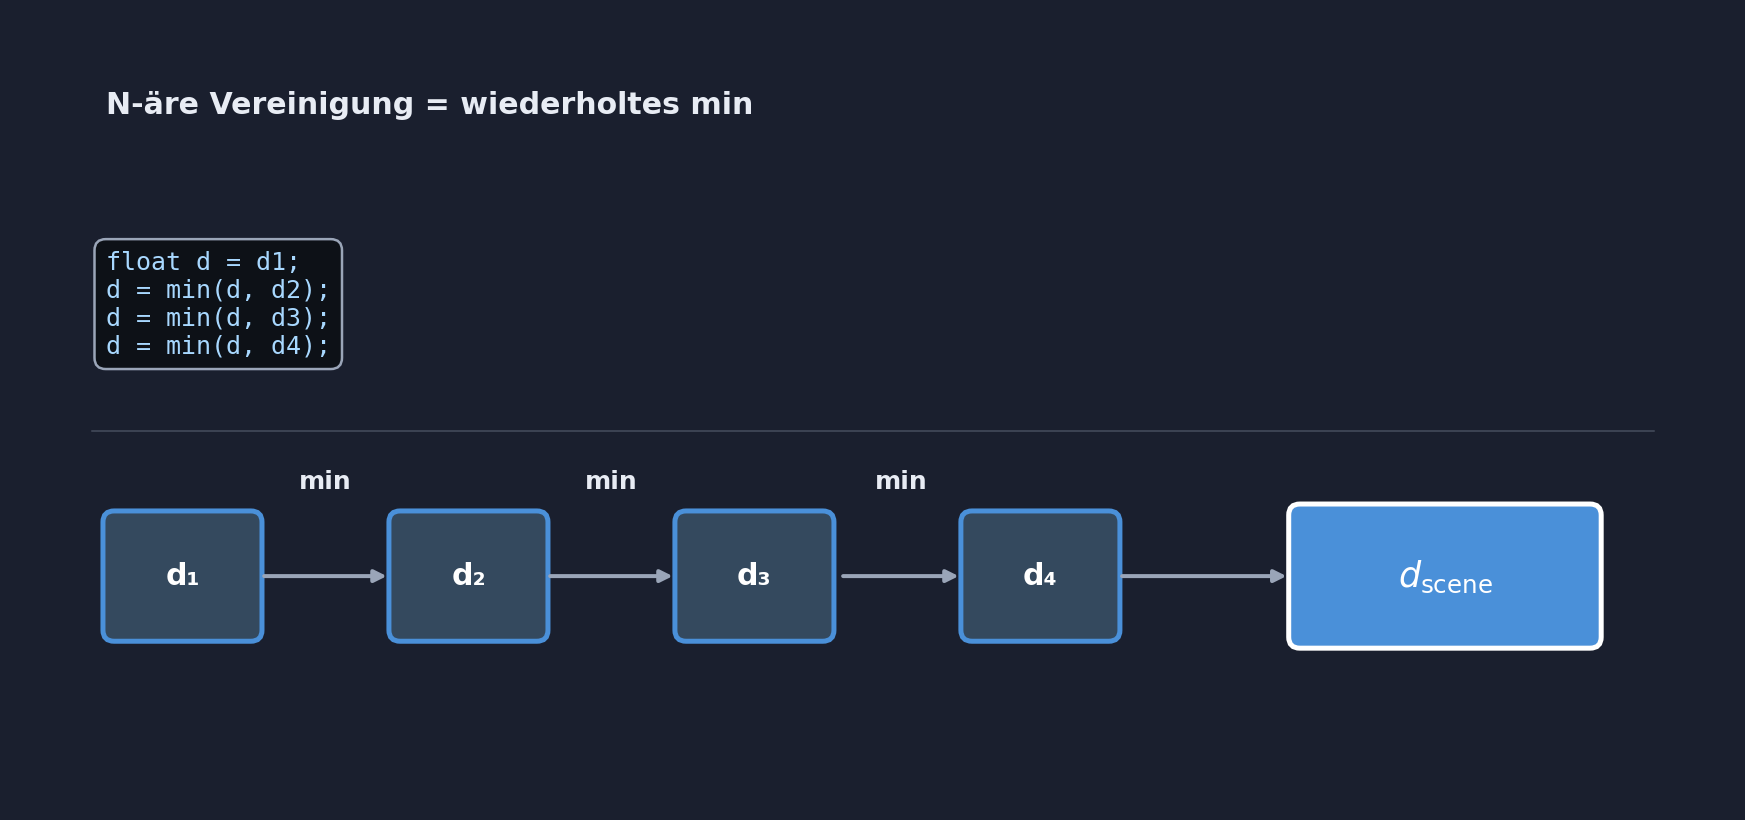
\includegraphics[width=0.88\linewidth,height=\textheight,keepaspectratio]{assets/diagrams/06-nary-union-chain.png}

\vspace{0.3em}

Mehrere Objekte = \textbf{assoziatives} Verketten derselben Operation
(Reihenfolge bei Union/Diff egal).

\section{Beispiel: gerenderte Szene}\label{beispiel-gerenderte-szene}

\subsection{Vom Baum zum Bild}\label{vom-baum-zum-bild}

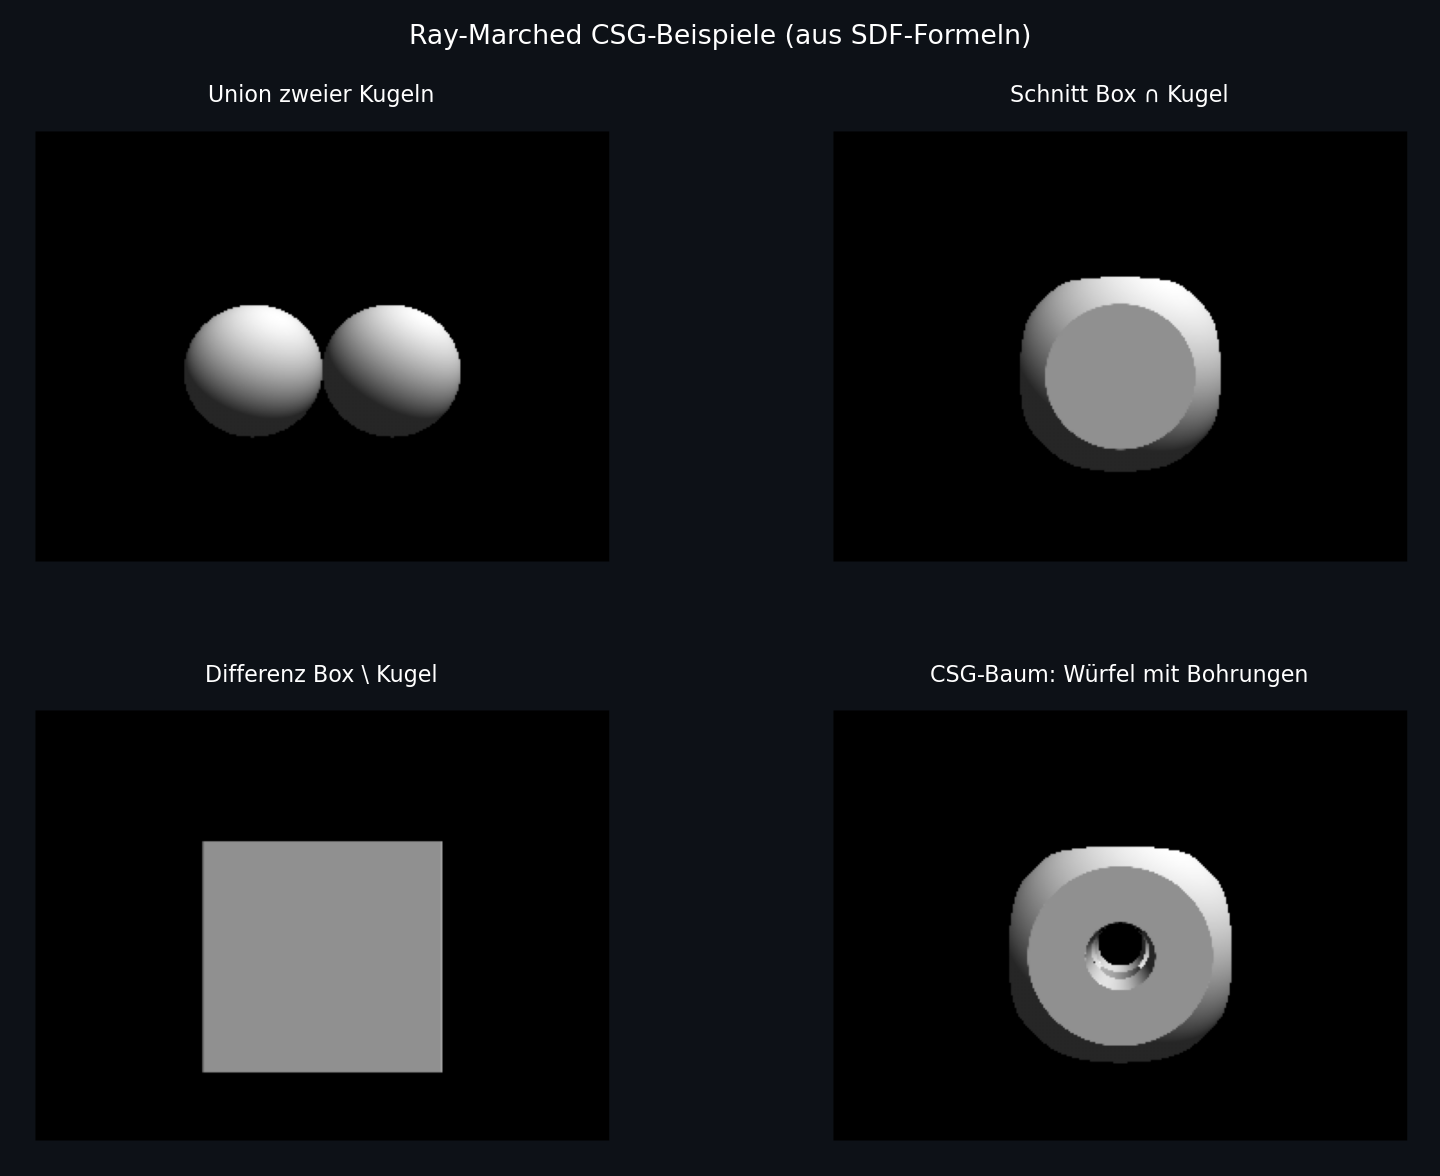
\includegraphics[width=0.95\linewidth,height=\textheight,keepaspectratio]{assets/diagrams/10-render-panel.png}

\footnotesize

Software-Raymarch aus denselben Formeln --- kein Mesh. Rechts unten: der
FreeCAD-ähnliche CSG-Baum.

\subsection{Vollständiger
Shader-Ausschnitt}\label{vollstuxe4ndiger-shader-ausschnitt}

\begin{Shaded}
\begin{Highlighting}[]
\DataTypeTok{float} \FunctionTok{sdCylinder}\OperatorTok{(}\DataTypeTok{vec3}\NormalTok{ p}\OperatorTok{,} \DataTypeTok{float}\NormalTok{ h}\OperatorTok{,} \DataTypeTok{float}\NormalTok{ r}\OperatorTok{)} \OperatorTok{\{} \CommentTok{/* ... */} \OperatorTok{\}}

\DataTypeTok{float} \FunctionTok{scene}\OperatorTok{(}\DataTypeTok{vec3}\NormalTok{ p}\OperatorTok{)} \OperatorTok{\{}
  \DataTypeTok{float}\NormalTok{ holes }\OperatorTok{=} \BuiltInTok{min}\OperatorTok{(}\BuiltInTok{min}\OperatorTok{(}\FunctionTok{sdCylinder}\OperatorTok{(}\NormalTok{p}\OperatorTok{.}\FunctionTok{zxy}\OperatorTok{,} \FloatTok{1.2}\OperatorTok{,} \FloatTok{0.22}\OperatorTok{),}
                        \FunctionTok{sdCylinder}\OperatorTok{(}\NormalTok{p}\OperatorTok{.}\FunctionTok{yzx}\OperatorTok{,} \FloatTok{1.2}\OperatorTok{,} \FloatTok{0.22}\OperatorTok{)),}
                    \FunctionTok{sdCylinder}\OperatorTok{(}\NormalTok{p}\OperatorTok{,}       \FloatTok{1.2}\OperatorTok{,} \FloatTok{0.22}\OperatorTok{));}
  \DataTypeTok{float}\NormalTok{ core  }\OperatorTok{=} \BuiltInTok{max}\OperatorTok{(}\FunctionTok{sdBox}\OperatorTok{(}\NormalTok{p}\OperatorTok{,} \DataTypeTok{vec3}\OperatorTok{(}\FloatTok{0.75}\OperatorTok{)),}
                    \FunctionTok{sdSphere}\OperatorTok{(}\NormalTok{p}\OperatorTok{,} \FloatTok{0.95}\OperatorTok{)} \OperatorTok{{-}} \FloatTok{0.0}\OperatorTok{);}
  \KeywordTok{return} \BuiltInTok{max}\OperatorTok{(}\NormalTok{core}\OperatorTok{,} \OperatorTok{{-}}\NormalTok{holes}\OperatorTok{);}  \CommentTok{// Differenz}
\OperatorTok{\}}
\end{Highlighting}
\end{Shaded}

\section{Erweiterungen (kurz)}\label{erweiterungen-kurz}

\subsection{Was noch mit derselben Idee
geht}\label{was-noch-mit-derselben-idee-geht}

\textbf{Glatte CSG} --- scharfe Kanten durch polynomiale Mischung
ersetzen:

\begin{Shaded}
\begin{Highlighting}[]
\DataTypeTok{float} \FunctionTok{smoothUnion}\OperatorTok{(}\DataTypeTok{float}\NormalTok{ d1}\OperatorTok{,} \DataTypeTok{float}\NormalTok{ d2}\OperatorTok{,} \DataTypeTok{float}\NormalTok{ k}\OperatorTok{)} \OperatorTok{\{}
  \DataTypeTok{float}\NormalTok{ h }\OperatorTok{=} \BuiltInTok{clamp}\OperatorTok{(}\FloatTok{0.5} \OperatorTok{+} \FloatTok{0.5}\OperatorTok{*(}\NormalTok{d2}\OperatorTok{{-}}\NormalTok{d1}\OperatorTok{)/}\NormalTok{k}\OperatorTok{,} \FloatTok{0.0}\OperatorTok{,} \FloatTok{1.0}\OperatorTok{);}
  \KeywordTok{return} \BuiltInTok{mix}\OperatorTok{(}\NormalTok{d2}\OperatorTok{,}\NormalTok{ d1}\OperatorTok{,}\NormalTok{ h}\OperatorTok{)} \OperatorTok{{-}}\NormalTok{ k}\OperatorTok{*}\NormalTok{h}\OperatorTok{*(}\FloatTok{1.0}\OperatorTok{{-}}\NormalTok{h}\OperatorTok{);}
\OperatorTok{\}}
\end{Highlighting}
\end{Shaded}

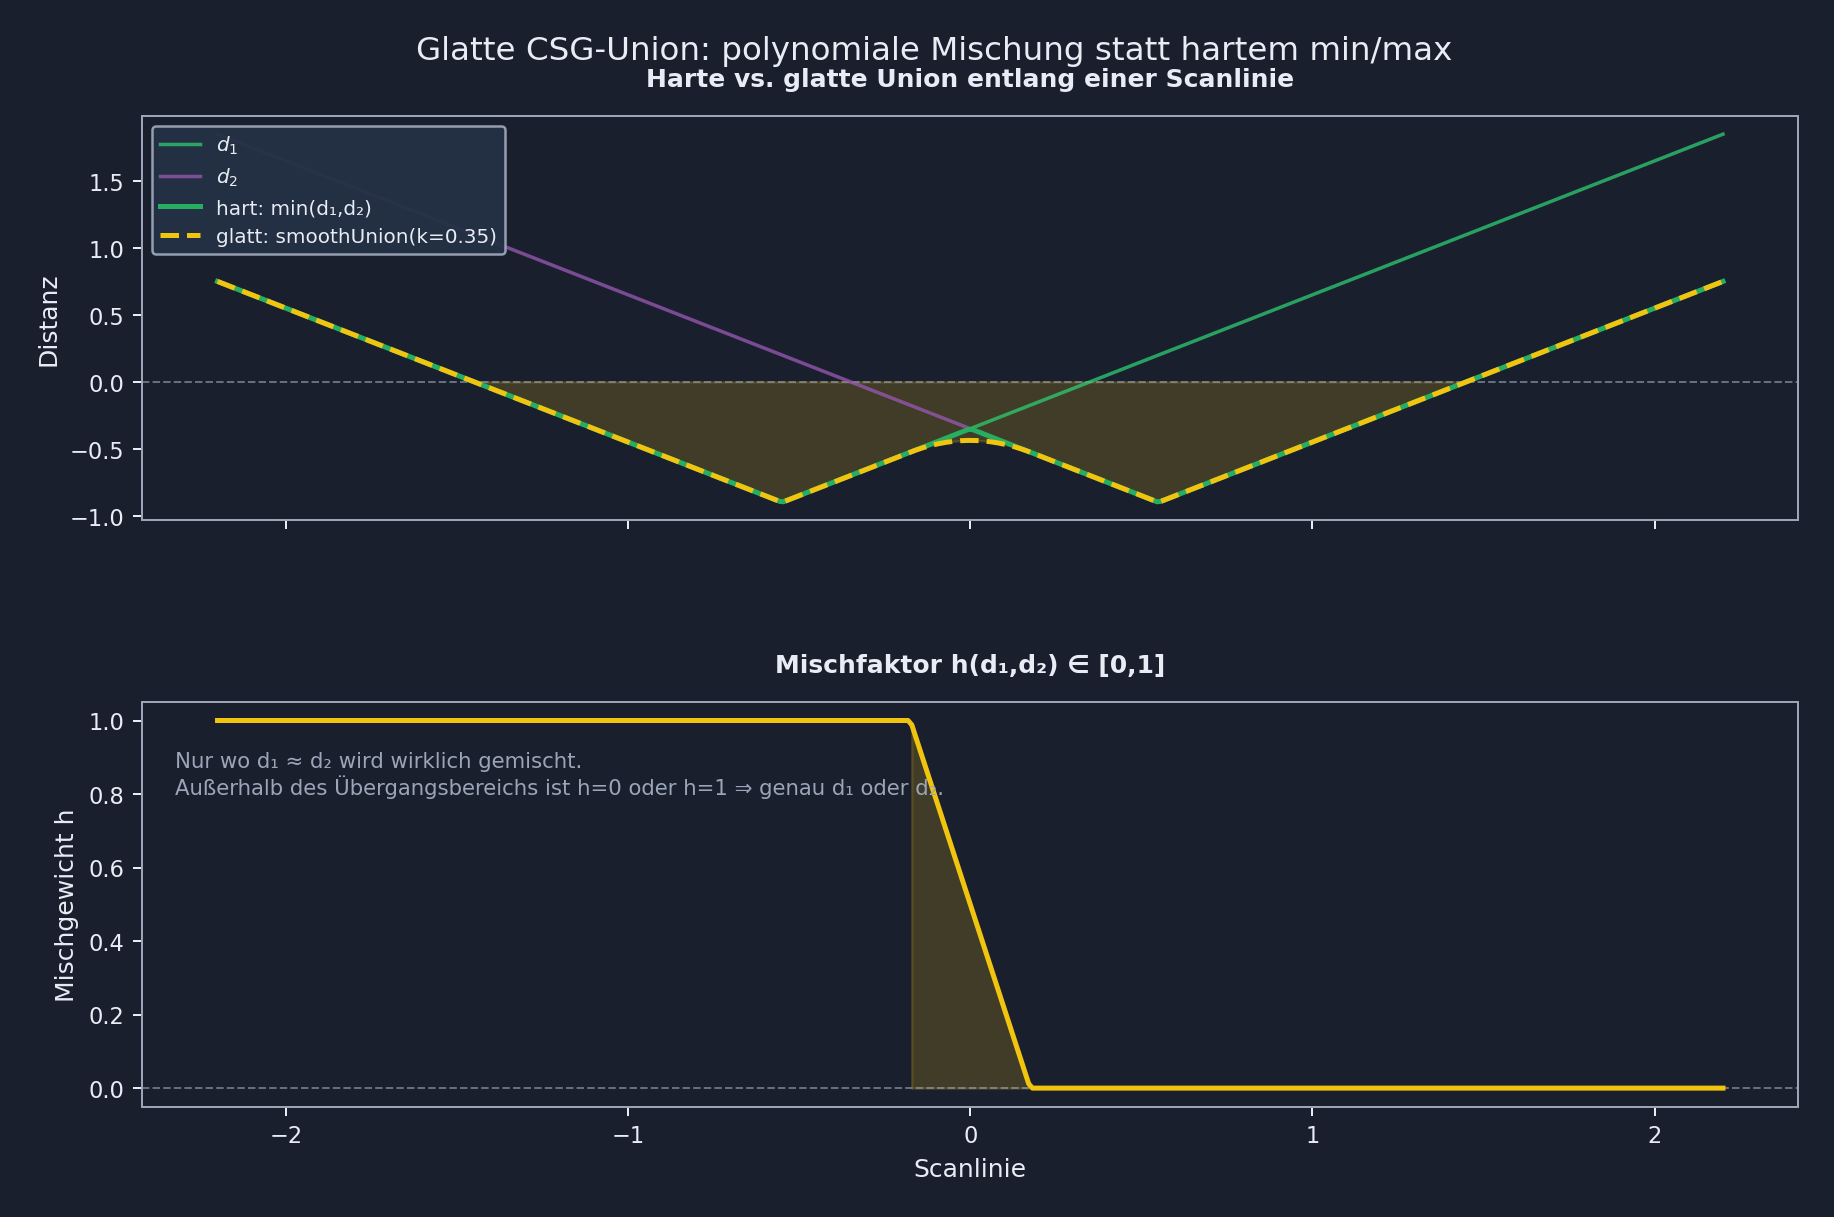
\includegraphics[width=0.72\linewidth,height=\textheight,keepaspectratio]{assets/diagrams/07-smooth-union.png}

\subsection{Weitere Anwendungen}\label{weitere-anwendungen}

\begin{itemize}
\tightlist
\item
  \textbf{Verschachtelung beliebiger Tiefe} --- CSG-Bäume, nicht nur
  zwei Operanden
\item
  \textbf{Domain-Operationen} --- Translation, Rotation, Skalierung
  \emph{vor} der SDF-Auswertung
\item
  \textbf{Wiederholung} --- \texttt{mod(p,\ spacing)} für Gitter/Tunnel
  (kein boolesches Op, aber kombinierbar)
\item
  \textbf{Performance:} eine Funktion \texttt{map(p)} ---
  GPU-freundlich, parallel pro Pixel
\end{itemize}

\vspace{0.5em}

\textbf{Kernbotschaft:} CSG auf SDFs = boolesche Mengenalgebra,
umgesetzt als punktweise min/max --- die Brücke zwischen
„Modellierungsbaum'' und „Ray-Marching-Schleife''.

\section{Zusammenfassung}\label{zusammenfassung}

{\def\LTcaptype{none} % do not increment counter
\begin{longtable}[]{@{}ll@{}}
\toprule\noalign{}
\endhead
\bottomrule\noalign{}
\endlastfoot
Union & \(\min(d_1, d_2)\) --- nähere Fläche \\
Schnitt & \(\max(d_1, d_2)\) --- beide innen \\
Differenz & \(\max(d_1, -d_2)\) --- invertiertes \(B\) \\
Szene & verschachtelter Ausdrucksbaum \\
Rendering & \texttt{map(p)} in der Ray-Marching-Schleife \\
\end{longtable}
}

\vspace{0.8em}

\centering

\large Fragen?




\end{document}
